\chapter{Funktionsweise \label{chap_funktionsweise}}
\ac{ITS} besteht aus verschiedenen Komponenten. Diese Komponenten können mobil oder stationär sein. Die Grafik \ref{fig:funktionsweise_komponentenueberblick} gibt einen Überblick über die in \ac{ITS} verwendeten Komponenten. Jede dieser Komponenten enthält eine \ac{ITS} Station.

\begin{figure}
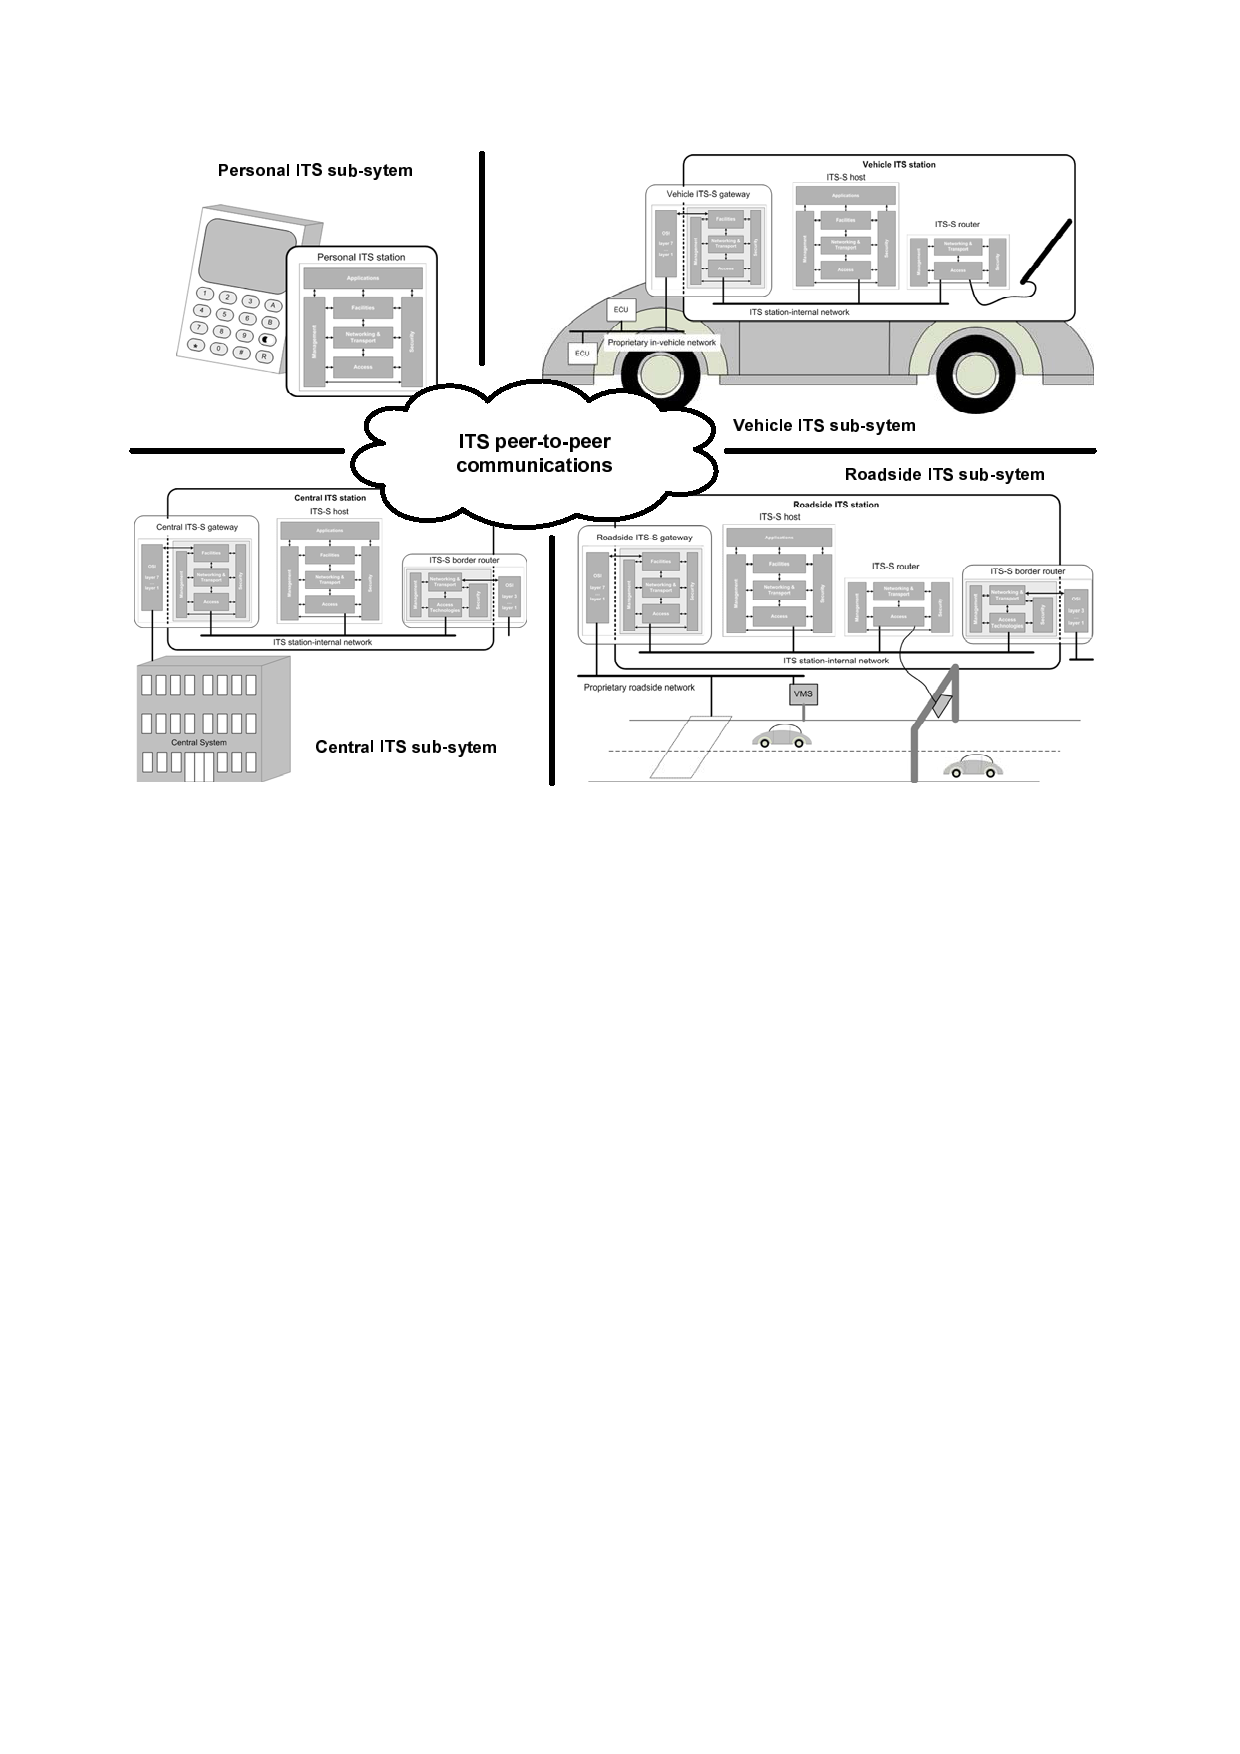
\includegraphics[width=0.8\textwidth]{content/images/01_funktionsweise/ueberblick-ITS-subsystems.pdf}
\caption{Überblick über die Komponenten \cite{etsi2010302}}
\label{fig:funktionsweise_komponentenueberblick}
\end{figure}

\section{Personal subsystem and station}
\ac{PSS} stellen die Funktionalitäten von \ac{ITS} in Geräten zur Verfügung, die in der Hand gehalten werden können. Der Standard nennt hierzu \ac{PDA} oder Mobiltelefone als Beispiel. Sie können als eigenständige Komponente dienen, oder als Teil einer anderen Komponente arbeiten.

\section{IRS}

\section{IVS}

\section{ICS}
